Antes de hablar de Sistemas Satelitales hay que saber que es un satélite y algunos aspectos básicos para entender el resto. Según la difinicion corriente, ``es un objeto en el espacio que orbita o da vueltas alrededor de un objeto mas grande'', pueden ser de dos tipos: \textbf{naturales} (como la luna) o \textbf{artificiales} (como la estación espacial Internacional). El segundo es el que tiene la capacidad de amplificar las señales. 
\\${ }$\\
Desde los años 50s se intentó de establecer sistemas de comunicación mediante el rebote de señales sobre globos meteorológicos. Lo malo era que las señales que se recibian eran demasiado débiles. Luego se intentó usar la luna para hacer rebotar las señales, pero tampoco funcionó. Aqui es cuando aparecen los satélites.
\subsubsection*{Estructura de un Satélite}
Podemos considerarlo como un repetidor de ondas (microondas) que contiene varios transpondedores, cada uno de los cuales escucha cierta porción del espectro, amplifica la señal y la retransmite en otra frecuencia. Esto se llama tubo doblado.
\subsubsection*{Estructura Física}
\begin{itemize}
\item \textbf{Transpondedor:} Cambia de frecuencia, eliminar ruido y amplifica el poder de la señal. Puede tener 20 o mas.
\item \textbf{Energía:} Baterias o paneles solares, estos ultimos se mueven en direccion al sol.
\item \textbf{Antena:} La mas comun es la reflectiva.
\item \textbf{Propulsor (Thruster):} Para mantener el satelite en su lugar. Esos son monitoreados por bases en la tierra. Controlan la posición orbital.
\end{itemize}
\subsubsection*{Funcionamiento}
Un satélite se mantiene en su órbita gracias al balance entre la gravedad y fuerza centrífuga. Cuando es lanzado tiene la suficiente velocidad para entrar en este balance. Un satélite que este mas cerca de la tierra necesita mas velocidad para no ser atraído y como no hay aire, no hay resistencia, por lo que continuará girando. 
\subsection*{Orbitas}
Los satelites son colocados en ciertas orbitas alrededor de la tierra, y estas son:
\begin{itemize}
\item \textbf{Low Earth Orbit (LEO):} 160 a 2000 $Km$ (Periodo $\sim$1.5hrs).
\item \textbf{Medium Earth Orbit (MEO):} 2000 a $<$35786$Km$ (Periodo 12hrs).
\item \textbf{Geosynchronus Earth Orbit (GSO):} 35789$Km$ (23hrs 56min 4seg).
\item \textbf{Geostationary Earth Orbit (GEO):} 35789$Km$ (23hrs 56min 4seg). Esta orbita esta unicamente en la línea del Ecuador.
\end{itemize}
Hay una región llamada Cinturón de Van Allen, una región con particulas altamente cargadas. que podrían dañar los componentes del satélites.

\begin{figure}[H]
\centering
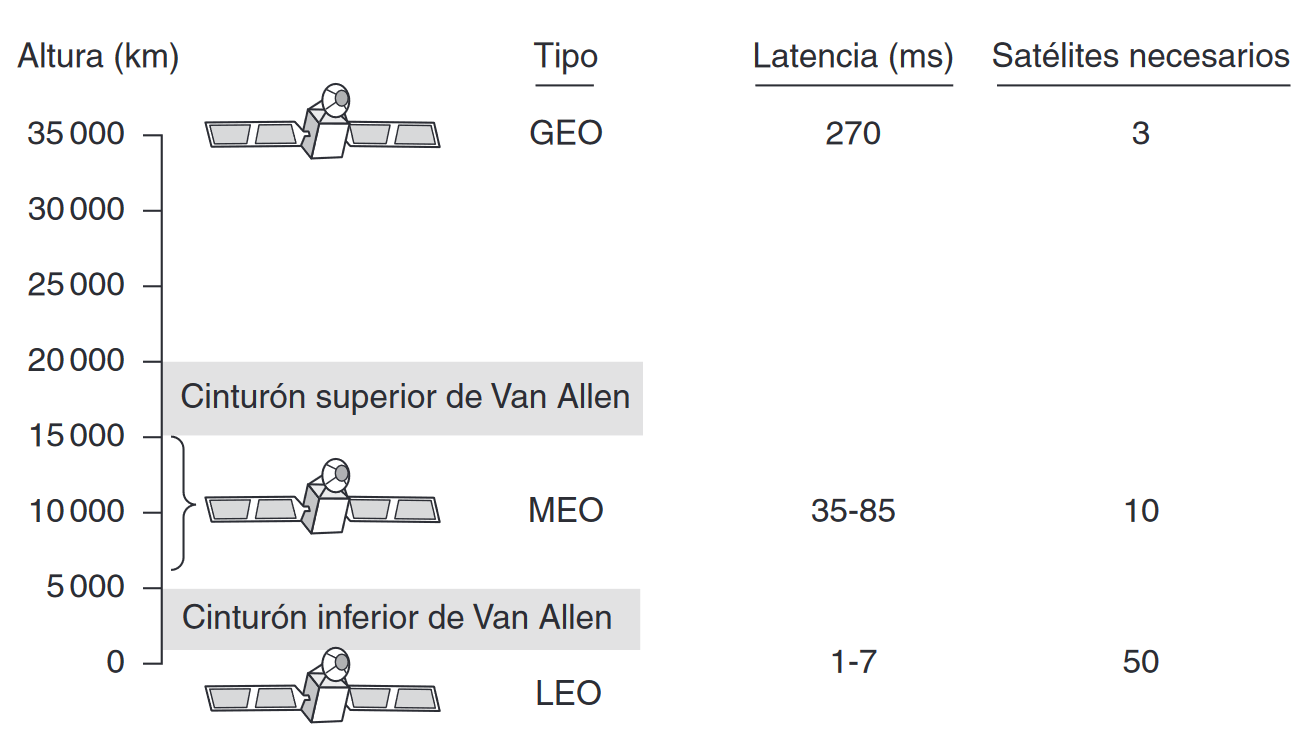
\includegraphics[page=1,scale=0.7]{SATELITES.png}
\caption{Alturas a las que se encuentran los satélites. \textit{(Redes de Computadoras, Tanenbaum 4ta Edición, Pagina 101)}}
\end{figure}

\subsection*{Satélites Geoestacionarios}
Estos satélites son colocados a $\sim$35800$Km$ en una órbita ecuatorial circular, esto hace que parezca que está girando con la tierra. Con la invención del transistor fue posible lanzar el primer satélite de comunicación satelital (1962). Estos pueden estar conectados con hasta 1 grado de separación, esto quiere decir que puede haber hasta 360 satélites. \\${ }$\\
En los primeros satelites la división de transpondedores era estatica, simplemente se dividia en bandas fijas de frecuencia. Hoy en dia se usa WDM y WDT. \\${ }$\\
Los primeros satélites \textbf{GEO} tenian un haz que cubría $1/3$ de la tierra (huella), con el tiempo esto cambió y se pueden hacer puntuales (forma elíptica y 100$Km$ area). 
\subsubsection*{Aplicaciones}
\begin{itemize}
\item Predicciones climáticas
\item Comunicación
\item Propositos Militares
\item GPS
\end{itemize}
También hay que tener en cuenta los \textbf{Satélites Geosincronos} cuya diferencia con los \textbf{GEO} es que estos no estan alineados al Ecuador, por lo que tienen cierta inclinación al respecto.

\subsection*{Satélites de Órbita Terrestre Media}
En altitudes mas bajas que los anteriores, se desvian lentamente en longitud y tardan 12 hrs para dar la vuelta a la tierra, es por esto que tienen menor huella y requieren transmisiones menos poderosas.
\subsubsection*{Aplicaciones}
\begin{itemize}
\item GPS
\item Glonass (Gloval Nav. Satellite System, Russia). 26 Satelites, 24 Activos.
\item Galileo (Global Nav. System, Union Europea). 30 Satelites, 22 Activos.
\end{itemize}
\subsection*{Satélites de Órbita Terrestre Baja}
Estos se encuentran a una altitud aun mas baja. Debido a su rapido movimiento se necesita una gran cantidad para un sistema completo, las estaciones terrestres no necesitan mucha potencia, el costo de lanzamiento es mas económico.

\begin{figure}[H]
\centering
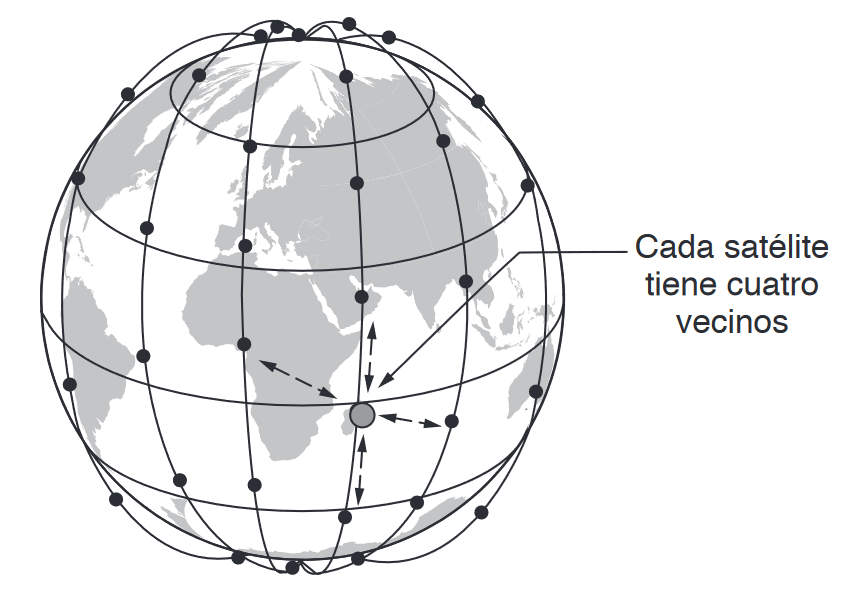
\includegraphics[page=1,scale=0.7]{SATELITES2.png}
\caption{Satélites Iridium \textit{(Redes de Computadoras, Tanenbaum 4ta Edición, Pagina 105)}}
\end{figure}

%\begin{figure}[H]
%\centering
%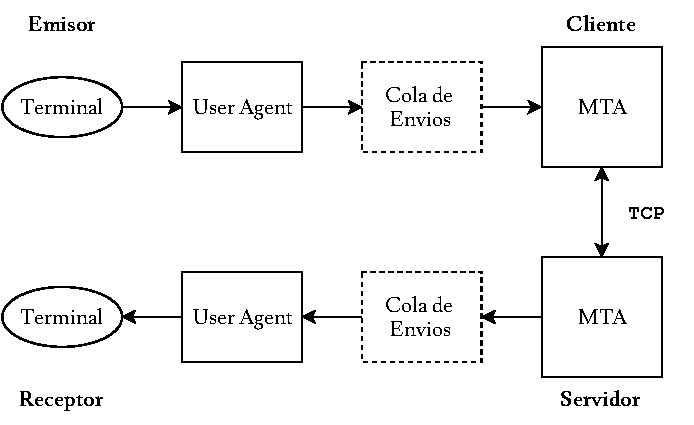
\includegraphics[page=1,scale=0.7]{SMTP.pdf}
%\caption{Esquema de funcionamiento de SMTP}
%\end{figure}
